% ICMC 2001 paper template for Latex2e.

% Points to note:
%    Please use \paragraph instead of \subsubsection -- see discussion below.
%    See comments in the References section on how to do citations.

\documentclass[10pt,a4paper]{article}
\usepackage{amsmath,amssymb,amscd,epsfig}
\usepackage{fullpage}
\usepackage{times}
\usepackage{chicago}                    % for "(Author, year)" cite style.
\usepackage{indentfirst}                % indent para after headings.
% \usepackage{url}                      % (handy if you reference a URL.)

%\usepackage{fullpage}
\usepackage{ifthen}
%% Should figures be compiled?
\newboolean{nofigures} % initially false ==> compile with figures
% comment out the following line to compile without figures
%\setboolean{nofigures}{true} 

%\usepackage{boxedminipage}
\usepackage{theorem}
{\theorembodyfont{\rmfamily} 
 \newtheorem{definition}{Definition}[section]
 \newtheorem{lemma}{Lemma}[section] % Lemmas are for proving theorems and facts
 \newtheorem{prop}{Proposition}[section] % Props state any new results of this document
 \newtheorem{fact}{Fact}[section]   % Facts are for less important, well-known results
 \newtheorem{example}{Example}[section]   
 \newtheorem{theorem}{Theorem}[section]  % Theorems are for important, well-known results
 {\theoremstyle{marginbreak}  
   \newtheorem{define}{}  % This definition style is for the glossary
    \newtheorem{Theorem}{Theorem}[subsection]  % Theorems are for important, well-known results
 }
}
\renewcommand{\thedefine}{}


% \setlength{\oddsidemargin}{-0.25in}     % Latex has one-inch "driver margin"
% \setlength{\evensidemargin}{-0.25in}  % (shouldn't be necessary)
\setlength{\textwidth}{160mm}             % 
\setlength{\textheight}{247mm} 
\setlength{\columnsep}{0.25in}
\setlength{\parindent}{0.2in}

\raggedbottom                           % better than inter-para spaces, I say.

%-------------------------------------------------------------
% Definitions.
% ------------
\def\HOME{/home/moonchild/pub/research/dsp/DeMeo/notes}
\def\R{\mathbb{R}}    % real numbers 
\def\Z{\mathbb{Z}}    % real numbers 
\def\C{\mathbb{C}}    % complex numbers 
\def\e{\mathrm{e}}    % exponential
% Two notations for real part of a complex number
   \def\Real{\mbox{Re}}  %\def\Real{\Re}
% Two notations for integration over R
   \def\integral{\int_{-\infty}^{\infty}}
     %\def\integral{\int_{-\infty}^{+\infty}} 
% Operator Theory
   \def\A{\operatorname{A}}
   \def\E{\operatorname{E}}
   \def\H{\operatorname{H}}
   \def\I{\operatorname{I}}
   \def\P{\operatorname{P}}
   \def\Per{\operatorname{Per}}
   \def\pv{\operatorname{pv}}
   \def\S{\operatorname{S}}
   \def\T{\operatorname{T}}
   \def\W{\operatorname{W}}
   \def\Hilbert{\mathcal{H}}
   \def\Hone{\mathcal{H}_1}
   \def\Htwo{\mathcal{H}_2}
   \def\Banach{\mathcal{B}(\Hilbert,\Hilbert)}
   \def\Banachonetwo{\mathcal{B}(\Hone,\Htwo)}
   \def\Banachtwoone{\mathcal{B}(\Htwo,\Hone)}
   \def\Lone{L^1}
   \def\Ltwo{L^2}
   \def\ltwo{\ell^2}
   \def\LoneR{L^1(\mathbb{R})}
   \def\LtwoR{L^2(\mathbb{R})}
   \def\ltwoR{\ell^2(\mathbb{R})}
   \def\Null{\mathcal{N}}  % nullspace
% Signals, Time-Frequency shifts, etc.
   \def\scale{\frac{1}{\sqrt{s}}}
   \def\transcale{\left(\frac{t-u}{s}\right)}
   \def\xpull{x_{\frac{\tau}{2}, -\frac{\xi}{2}}}
   \def\xpush{x_{-\frac{\tau}{2}, \frac{\xi}{2}}}
   \def\xpullpush{x_{\frac{\tau}{2}, \frac{\xi}{2}}}
   \def\xpushpull{x_{-\frac{\tau}{2}, -\frac{\xi}{2}}}
   \def\xfpull{x_{-\frac{\Delta\nu}{2}}}
   \def\xfpush{x_{\frac{\Delta\nu}{2}}}
   \def\apull{a_{-}}
   \def\apush{a_{+}}

   \def\ytnu{y_{t,\nu}}
   \def\ytnut{\tilde{y}_{t,\nu}}
   \def\half{{\scriptstyle \frac{1}{2}}}
   \def\halftau{{\scriptstyle \frac{\tau}{2}}}
   \def\halfxi{{\scriptstyle \frac{\xi}{2}}}
   \def\halfnu{{\scriptstyle \frac{\nu}{2}}}
   \def\halfDnu{{\scriptstyle \frac{\Delta\nu}{2}}}

   \def\xtpull{x\left(t+\halftau\right)}
   \def\xtpush{x\left(t-\halftau\right)}
%   (shouldn't need this) \def\xtpullconj{x^*\left(t+\halftau\right)}
   \def\xtpushconj{x^*\left(t-\halftau\right)}
   \def\Xtpull{X\left(\nu+\halfxi\right)}
   \def\Xtpush{X\left(\nu-\halfxi\right)}
   \def\Xtpullconj{X^*\left(\nu+\halfxi\right)}
%   (shouldn't need this) \def\Xtpushconj{X^*\left(\nu-\halfxi\right)}

   \def\ytpull{y\left(t+\halftau\right)}
   \def\ytpush{y\left(t-\halftau\right)}
%   (shouldn't need this) \def\ytpullconj{y^*\left(t+\halftau\right)}
   \def\ytpushconj{y^*\left(t-\halftau\right)}
   \def\Ytpull{Y\left(\nu+\halfxi\right)}
   \def\Ytpush{Y\left(\nu-\halfxi\right)}
   \def\Ytpullconj{Y^*\left(\nu+\halfxi\right)}
%   (shouldn't need this) \def\Ytpushconj{Y^*\left(\nu-\halfxi\right)}

% Language
   \def\FT{Fourier transform}
   \def\WT{Wigner transform}
   \def\WV{Wigner-Ville}

%%-------------------------------------------------------------
\begin{document}

\twocolumn

\title{\textbf{Characterizing Musical Signals \\
with Wigner-Ville Interferences}}
\author{William J. DeMeo\\
{\small {\tt williamdemeo@yahoo.com}}}
\date{}     % no date
\maketitle

\pagestyle{empty}          % no page numbers.
\thispagestyle{empty}      % yes, that includes not on the first page, either.

% do abstract by hand -- \begin{abstract} wouldn't conform to the guidelines.

\begin{center}
\large{\textbf{Abstract}}
\end{center}
% there's this annoying little indent here I can't properly eliminate, so...
\hspace*{-0.1in}                       % hackily cancel it out.
\noindent
\textit{
This paper presents a new characterization of musical signals which
may lead to better understanding about how such signals are perceived. 
We first consider some signal analysis methods which
facilitate measures of perceived qualities of music.  More precisely, we
consider a particular representation of signal energy on which to base a
quantitative measure of \emph{sensory dissonance}.  After defining sensory
dissonance in section~\ref{sec:consonance}, we describe a well known signal
decomposition method, the matching pursuit.  Thereafter, we consider one aspect of
signal energy which has been largely ignored in the literature -- the
Wigner-Ville interferences.  We explain why and how these interferences can be used
as the basis for a dissonance characterization of a musical signal.}
% -*- mode: LaTeX; tex-main-file: "../notes.tex"; -*-
%\begin{itemize}
%\item Synthesis -- Sethares (p.15), comp book (00.07.17), beige book (00.07.27)
%\item Tonal Fusion -- comp book (00.07.10)
%\item Spectral Dominance -- Hartmann (p.298) and beige book (00.07.11)
%\item Tonal Dissonance -- comp book (00.07.21)
%\item Wavelet Theory -- beige book (00.07.31, 00.08.01, 00.08.02)
%\end{itemize}
%\input{\HOME/intro/quote.tex}
\section{Introduction}
\subsection{DSP for Perception Analysis}
We begin by stating the two main objectives of this work.  Given a musical
signal, $x(t)$, we wish to:
\begin{enumerate}
\item \label{item:spectral} find useful time-frequency representations for
  analyzing the information content of $x(t)$, with the goal of characterizing
  perceptual properties of the signal;
\item \label{item:dissonance} %using the results of~\ref{item:spectral},
  find measures of qualities related to human perception of the signal;
  in particular derive a ``dissonance signature'' of $x(t)$. 
\end{enumerate}

In addressing (\ref{item:spectral}), we use the \emph{matching pursuit}
algorithm \cite{Mallat:1993}
to perform an atomic decomposition of the signal.  We then use this
decomposition as the basis for an energy characterization of the signal, given
by the \emph{Wigner-Ville distribution}.  This approach is not new.  However,
the literature employing this strategy ignores the interference structure of
the Wigner-Ville distribution.  We retain these interference terms as they are
the focus of our approach to the second objective stated above.

The novel contribution of this paper is consideration of how the interference
terms of the Wigner-Ville decomposition can be used as the basis for a
dissonance measure of a musical signal.  For a simple composition of two pure
tones, there is a well known relation between the interference terms and
the sensory notion of ``beating'' -- i.e.~the effect caused by amplitude
modulations resulting from the composition of tones.  Since some measures of
sensory dissonance are motivated by the rate of such beating, this
suggests basing our dissonance characterization on the interference structure
of a musical signal.

\subsection{Sensory Dissonance}
The concept of \emph{sensory dissonance} was originally proposed
by Helmholtz~\citeyear{Helmholtz:1877}, and further developed by Plomp and 
Levelt~\citeyear{Plomp:1965}, and Sethares~\citeyear{Sethares:1997}.
%Though we consider these studies in greater detail in
%sections~\ref{sec:consonance} and~\ref{sec:disscurves}, 
What follows is a %description that motivates our alternative treatment of
description of dissonance that motivates our alternative treatment of
this concept.

In order to assess the intrinsic dissonance of a musical signal over a
small time interval, the aforementioned studies employ a function of
the signal's estimated frequency components over that interval.
This often provides a useful quantitative measure.  However, such a
function makes no attempt to account for other widely accepted notions
of dissonance.   
Perhaps the most obvious short-coming results from the point-wise
nature of this dissonance function.  That is, because it is
well localized in time, there is no way for the dissonance function to account
for \emph{melodic dissonance} of the signal.  The melodic
dissonance of a given segment of music depends on that 
segment's relation to its context.  In our present work, we
consider signal analysis methods that provide for
%estimates of
%instantaneous frequencies and analytic amplitudes of a signal, and use 
%these estimates to measure the dissonance properties of the
%signal.  A primary objective is the development of methods providing
more dynamic dissonance measures.  In particular, we wish to simultaneously
account for local, point-wise dissonance, as well as dissonance resulting from
the melodic contour of the signal.  

%\subsection{Spectral Analysis of Musical Signals}
%There is a vast literature on the spectral analysis of musical signals. The
%broad class of analysis methods that we consider here 
%consists of {\it time-frequency representations}.  The type of signal
%which concerns us is a {\it time series}, $x(t)$.  Usually we assume that
%periodicities play an important role in the structure of $x(t)$.  To study the
%signal from this point of view, we decompose it as a function of both time and
%frequency. Such a decomposition is what we mean by a time-frequency
%representation (TFR). 
%
%The two broad classes of TFR's which we consider are {\it atomic
%decompositions} and {\it energy distributions}.  The first decomposes a
%signal by ``projecting'' it onto the time-frequency space, thereby equating
%it with a weighted sum of basic elements in that space.
%Some more detailed discussion of atomic decompositions appears is
%section~\ref{sec:atomic}. 
%The second class of TFR's are the energy distributions, the primary
%objective of which is to represent a distribution of the signal's energy
%across the time-frequency plane.  We consider the energy distributions in
%section~\ref{sec:energy}. 
%
%Though atomic decompositions, such as wavelet and windowed Fourier techniques,
%can be effectively applied to non-stationary signals, they suffer from the
%adverse consequences of Heisenberg's uncertainty principle, manifested in a
%time-frequency resolution trade-off.  The more general distributions of
%section~\ref{sec:energy} can help us overcome this limitation.
%

% -*- mode: LaTeX; tex-main-file: "../notes.tex"; -*-
\section{Measures of Consonance}
In later sections, we consider signal analysis methods that are
particularly well suited to the type of musical analysis we wish to
perform.  Therefore, we should first consider %crucial that we have a good grasp of the
some of the musical ideas underlying and motivating our work.
The next section presents one such notion --
musical \emph{consonance}.  We also briefly discuss some existing
quantitative measures of this concept; the reader can find a more detailed
treatment in Sethares \citeyear{Sethares:1997}.
% (end: insert file synthesis.tex)

% (begin: insert file consonance.tex)
\subsection{Consonance and Dissonance}
\label{sec:consonance}
According to Tenney~\citeyear{Tenney:1988} and Sethares
\citeyear{Sethares:1997}, the historical usage of the term {\it
consonance} 
%(and its antonym, {\it dissonance}) 
can be classified according to five distinct categories:
%(see~\citeN{Sethares:1997} for more details):
\emph{melodic consonance} (CDC-1), \emph{polyphonic consonance} (CDC-2),
\emph{contrapuntal consonance} (CDC-3), \emph{functional consonance} (CDC-4),
\emph{sensory consonance} (CDC-5).  

In this paper, the focus is on CDC-1 and CDC-5, so we describe only these.
Briefly, \emph{melodic consonance} applies to successive melodic intervals and
describes these intervals as either consonant or dissonant depending on the
surrounding melodic context; it refers to relatedness of pitches sounded
successively, or the \emph{melodic contour}.  \emph{Sensory consonance}
equates consonance with smoothness and the absence of beats, and equates
dissonance with roughness and the presence of beats.

The definition of sensory consonance is based on the  phenomenon of
beats.  If two pure sine tones are sounded at almost the same
frequency, then beating occurs due to the interference between the
tones.  The beating becomes slower as the two frequencies approach
each other and disappears when they coincide.  Typically, slower  
beats are perceived as gentle and pleasant while fast beats are
perceived as rough and unpleasant. Observing that any sound can be
decomposed into sinusoidal partials, Helmholtz~\citeyear{Helmholtz:1877}
theorized that the perception of dissonance in a musical tone is
determined by the presence and quality of beats among the tone's
interacting partials. 

The present research effort is directed at the discovery of a
measure which might simultaneously quantify multiple notions of consonance.
In particular, we  would like to exploit the theory of \emph{sensory}
and \emph{tonal} consonance (CDC-2 and CDC-5)
of Plomp and Levelt~\citeyear{Plomp:1965} as well as its elaboration
in~\citeN{Sethares:1997}.  
%Some of this theory is described below in
%section~\ref{sec:disscurves}.  
Briefly, this theory employs functions called
\emph{dissonance curves} which measure the ``sensory'' dissonance, of
a complex tone at each particular instant in time.\footnote{Really, a
small interval of time is required to ascertain what pseudo-periodic
frequencies are present at a particular instant.}   
This provides a useful point-wise measure.
However, we would also like a measure that is dynamic and appeals to a
melodic sense of consonance, as in CDC-1.  For example, a dissonance curve
does not account for dissonance due to melodic changes from one complex tone
to the next.  

%\subsection{Dissonance Curves}
%\label{sec:disscurves}
%Two pure sine waves are both perceptible if the frequencies are well
%separated.  When the frequencies are close together, only one sine
%wave is heard (though possibly with beats).  By varying the frequency
%of one of the waves while keeping the other wave fixed, Plomp and
%Levelt~\cite{Plomp:1965} gathered data revealing subject's preferences
%for various frequency intervals.  An example of what these data
%indicate appears as a \emph{dissonance curve} in 
%Figure~\ref{fig:1DissCurve}. Methods for deriving such curves in
%practice are described in~\cite{Sethares:1997}.  These curves are 
%in stark contrast to existing musical theory.  In particular they imply 
%that, in terms of sensory dissonance, intervals such as the major 7th and
%minor 9th are almost indistinguishable from the octave.  This leads some 
%to argue that these data bear no relation to our notions of musical
%consonance. Regardless of whether they have a direct influence on our 
%ideas about musical intervals, dissonance curves provide a way to measure
%the intervals among \emph{pure sine waves}.  Therefore, they can be 
%useful when analyzing a musical signal that has been decomposed into 
%its spectral components.
%
%\begin{figure}
%\ifthenelse{\boolean{nofigures}}{}{
%%             \pdfimage
%%             width 120 mm 
%%             height 70 mm
%%             {\HOME/figures/1DissCurve.png}
%\centering  
%\includegraphics[width=120mm, height=70mm]{\HOME/figures/1DissCurve}
%}
%\caption{{\small Two sine waves are sounded simultaneously.  Typical
%perceptions include pleasant beating (at small frequency ratios),
%roughness (at middle ratios), and separation into two tones (at first
%with roughness, and later without) for larger ratios.  the horizontal
%axis represents the frequency interval between the two sine waves,
%and the vertical axis is a normalized measure of ``sensory''
%dissonance.  The frequency of the lower sine wave is 400 Hz}}
%\label{fig:1DissCurve}
%\end{figure}
%
%% Leaving out this figure for now:
%%\begin{figure}
%\ifthenelse{\boolean{nofigures}}{}{
%%             \pdfimage
%%             width 120 mm 
%%             height 70 mm
%%             {\HOME/figures/3DissCurves.png}
%\centering  
%\includegraphics[width=120mm, height=70mm]{\HOME/figures/3DissCurves}
%}
%\caption{{\small Two sine waves are sounded simultaneously.  The
%horizontal axis represents the frequency interval between the two sine
%waves, and the vertical axis is a normalized measure of ``sensory''
%dissonance. The plot shows how the sensory consonance and dissonance
%change depending on the frequency of the lower tone.}}
%\label{fig:3DissCurves}
%\end{figure}
%% (end: insert file consonance.tex)

%%% NEWER (UNDERDEVELOPED) IDEAS %%%
%Recall equation~(\ref{eqn:sumpartials}) of section~\ref{sec:synthesis}
%in which a complex tone $x$ is modeled as a weighted sum of sinusoidal
%partials: 
%\[x(t) = \sum_{k=1}^K a_k(t) \cos(\phi_k(t))\]
%where the instantaneous frequency of the $k$th partial is
%%(cf.~\S~\ref{sec:instfreq}, equation~\ref{eqn:sumpartials}): 
%\[\omega_k(t) = \phi'_k(t) \geq 0.\]
%Suppose for simplicity that the set of $K$ instantaneous frequencies
%$\{\omega_k\}$ are known and constant over a small interval (instant)
%of time.  Then...
%%the relative dissonances among the frequencies in a complex
%%tone
%
%It is possible that a particular \emph{instant} in a piece of music
%will have a high sensory dissonance value but, because of this
%instant's relation to its context, the section of the piece containing
%this instant has a low total dissonance value.  We can create measures
%that act in this way.  Consider a simple succession of 3 instants of a
%musical piece represented by $\{S_0, S_1, S_2\}.$  Let $\|\cdot\|$ be
%the measure of dissonance of $S_k.$  It is possible ...


% -*- mode: LaTeX; tex-main-file: "../notes.tex"; -*-
% (begin: insert file ambiguity.tex)
%\subsection{Quadratic Time-Frequency Energy\protect\footnotemark}
%\footnotetext{Mallat~\cite{Mallat:1998} (p.107),
%Mertins~\cite{Mertins:1999} (p.265)} 
\section{Energy Distributions}
\label{sec:energy}
Wavelet and windowed Fourier transforms are computed by
correlating the signal with families of time-frequency atoms.  The
time and frequency resolution of these transforms is thus limited by
the time-frequency resolution of the corresponding atoms.  Ideally,
one would like to define a density of energy in a time-frequency
plane with no loss of resolution.  This section presents a
different class of time-frequency representation (TFR) which is not
restricted by the uncertainty principle.  

%\footnotetext{Mertins~\cite{Mertins:1999} (p.265)}
The \emph{Wigner-Ville TFR} is computed by
correlating $x$ with a time and frequency translation of itself.
(Below we refer to the Wigner-Ville TFR simply as 
% the ``\WV'' and, sometimes, as 
the ``\WT.'')  Though it yields some remarkable
properties, the quadratic from of this representation is also 
considered a drawback which limits its application because of the inevitable
cross terms that appear in quadratic forms.  An attempt is usually made to 
attenuate these so-called
``interference terms'' by performing a time-frequency averaging, but this 
procedure results in a loss of resolution. It is not hard to show
that the spectrogram, the scalogram, and all squared time-frequency
decompositions can be written as time-frequency averagings of the
\WT; see, e.g., Mallat~\citeyear{Mallat:1998}.

%Although the \WT\ does not yield positive distributions, it allows extremely
%good insight into signal properties within certain applications.

\subsection{Wigner Transform}
%\ifthenelse{\boolean{nofootnotes}}{\subsection{Wigner Transform}}
%{\subsection{Wigner Transform\protect\footnotemark}
%\footnotetext{Mertins~\cite{Mertins:1999} (p.265)}}
%The ambiguity function represents the signal energy %of the signal 
%in the {\it frequency-time} plane.  We now transform this
%representation into the {\it time-frequency} plane.
\label{sec:wigner}
The quadratic form\footnote{Integrals are over the entire real line unless
  otherwise noted.}
\begin{equation*} %\label{eqn:WignerVille}
\W_x(t,\nu) = 
%\integral 
\int \xtpull \xtpushconj e^{-i2\pi \tau\nu}\,d\tau
\end{equation*}
is known as the \emph{Wigner-Ville distribution}, or \emph{\WT}.
It is the one-dimensional \FT\ of
$\phi_x(t,\tau) = \xtpushconj \xtpull$, with respect to $\tau$.
The function $\phi_x$ has a Hermitian symmetry in $\tau$, so the 
\WT\ is real valued. 
Also, as the two-dimensional \FT\ of the so called \emph{ambiguity function},  
\[
\A_{x}(\xi,\tau) = \int \xtpull \xtpushconj e^{i2\pi \xi t}\,dt
\]
the \WT\ satisfies
\begin{equation}\label{eq:ambig-ft}
\W_x(t,\nu) = %  \iint\limits_{\R^2} 
\int \A_x(\xi,\tau) e^{-i2\pi(\xi t + \nu\tau)}\,d\xi\,d\tau
\end{equation}

The \WT\ localizes the time-frequency structures of $x$.  If
the energy of $x$ is well concentrated in time around $t_0$ and in
frequency around $\nu_0$ then $\W_x$ has its energy centered at
$(t_0,\nu_0)$, with a spread equal to the time and frequency spread of
$x$. 
%\end{define}

\subsection{Interference Structure}% of Bilinear Transforms}
Because the \WV\ transform is a sesquilinear form of the signal, it
does not submit to the principle of linear superposition.  Instead, as in the
quadratic equation, $(a+b)^2 = a^2 + b^2 + ab + ba$, it is easy to verify that
\begin{align}
  \W_{x+y}(t,\nu) &= \W_x(t,\nu) + \W_y(t,\nu)\nonumber \\
      &+ \W_{xy}(t,\nu) +\W_{yx}(t,\nu) \label{eqn:Wignersum} 
\end{align}
where $\W_{xy}$ is the \emph{cross \WT\ } of the signals $x$ and $y$, which is
defined by 
%\begin{eqnarray*}
\begin{equation}
\label{eqn:crossWigner}
\W_{xy}(t,\nu) = \int \xtpull \ytpushconj e^{-i2\pi\nu\tau}\,d\tau 
\end{equation}
%\begin{align}\label{eqn:crossWigner}
%  \W_{xy}(t,\nu) &= \\
%& \integral \xtpull \ytpushconj e^{-i2\pi\nu\tau}\,d\tau \nonumber%\\
%  &=& \integral \Xtpush \Ytpullconj e^{-i2\pi\xi t}\,d\xi\nonumber
%\end{eqnarray*}\end{align}

%%It can also be shown that~(\ref{eqn:crossWigner}) is the
%%two-dimensional \FT\ of the \emph{cross ambiguity function},
%%which is defined by 
%%%\begin{eqnarray}\label{eqn:crossAmbiguity}
%%\[  \A_{xy}(\xi,\tau) = \integral \xtpull \ytpushconj e^{i2\pi \xi t}\,dt\]%\\
%%%   &=& \integral \Xtpush \Ytpullconj e^{i2\pi \xi t}\,dt\nonumber \\
%%%\end{eqnarray}

We define the \emph{interference term} of
equation~(\ref{eqn:Wignersum}) by
%\begin{eqnarray*}
%  I_{xy}(t,\nu) &=& \W_{xy}(t,\nu) + \W_{yx}(t,\nu) \\
%                 &=& 2\,\Real\left[\W_{xy}(t,\nu)\right]
%\end{eqnarray*}
\begin{align*}
  I_{xy}(t,\nu) &= \W_{xy}(t,\nu) + \W_{yx}(t,\nu)\\
 &= 2\,\Real\left[\W_{xy}(t,\nu)\right]
\end{align*}
This real valued function creates non-zero values at
interesting locations of the time-frequency %$(t,\nu)$ 
plane. 

More generally, for any linear combination of signal components,
\[
  x(t) = \sum_{n=1}^N a_n x_n(t)
\]
the \WT\ is
%\begin{equation}
\begin{align}
  \W_{x} &= \sum_{n=1}^N|a_n|^2 \W_{x_n}(t,\nu) \label{eq:WignerSum} \\
 &+ 2\sum_{n=1}^{N-1}\sum_{k=n+1}^N\,
                 \Real\left[a_n a_k^* \W_{x_nx_k}(t,\nu)\right]
\nonumber
%\end{equation}
\end{align}
Hence, for a signal with $N$ components, the \WT\ contains 
$N(N-1)/2$
additional components.  They result from the interaction of different
components of the signal, and are called ``interference terms'' for
two reasons.  First, the mechanism of their creation is analogous to
the usual interferences that can be observed for physical waves.  A
second reason for this terminology lies in the
effect that these terms can have on the %concerning the readability of a
time-frequency diagram of the signal energy.  As they amount to a
combinatorial proliferation of additional, ``specious'' signal
components, they can inhibit our ability to discern ``true'' signal 
components in the diagram.  

The presence of cross terms in a \WT\ can be regarded as a
natural consequence of its bilinear structure.  This very structure is also
what leads to most of the good properties of the transform (such as
localization).    
No matter whether one views the cross terms as helpful or hindering,
it is important to understand fully the mechanism of their creation.
This is indispensable for drawing the correct interpretation from the 
representation of an unknown signal, and for separating signal component
terms from interference terms if desired \cite{Flandrin:1999}.

In the present work, we study the
cross terms in order to understand how this measure of signal interference
relates to ``musical interference,'' i.e.~dissonance. 

%As a simple example, consider a well localized time-frequency
%atom, $x(t)$, centered at $t=0$, and the two atoms which are time and 
%frequency shifted versions of $x(t)$: 
%\[
%\xpull(t) = 
% \apull \xtpull e^{-i2\pi (\halfxi) t} \quad \text{ and }\quad  
%\xpush(t) = \apush \xtpush e^{i2\pi (\halfxi) t}
%\]
\subsection{Examples}
\label{sec:examples}
\def\a{\mathbf{a}}
\def\b{\mathbf{b}}
%We will start with some general terminology, but quickly proceed to
%specifics relevant to our application.  For a lucid treatment of the
%general theory of time-frequency representations on finite abelian groups,
%see~\cite{Tolimieri:1998}.  

%For some finite abelian group $A$, with dual $A^*$, consider the signal $x \in
%L(A)$, and define the \emph{Weyl-Heisenberg operator}
%$H : A \times A^* \rightarrow  L(A)$ by
%\[ 
%H(\a)x(t) = x_\a(t) = x(t-a)\langle t,a^* \rangle, \qquad t\in A
%\]
%for any pair $\a = (a,a^*) \in A\times A^*$.
%This simply provides a convenient notation for the common translation and
%modulation operation, a special case of which appears in~(\ref{eqn:transmod})
%below.\\ 
%\\
%{\bf Example}\\
For simplicity, suppose that $x \in L(\Z/N)$ represents an elementary signal
component, so that $x$ is a discrete periodic function of period $N$, defined
on the group of integers $\Z/N \simeq \{0,1,\ldots,N-1\}$.  In this
special case\footnote{For a more general, lucid treatment of the theory of
  time-frequency representations on finite abelian groups,
  see~\citeN{Tolimieri:1998}.} 
the so called \emph{Weyl-Heisenberg} operator is
$H : \Z /N \times \Z /N \rightarrow  L(\Z /N)$,
and is defined by
\begin{align*}
H(\a)x(n) &= x_\a(n) \nonumber\\
&= x(n-a_1)\;e^{i2\pi a_2n/N},
\quad x \in L(\Z/N) %\label{eqn:transmod}
\end{align*}
for any $\a = (a_1,a_2) \in \Z /N \times \Z /N$.

The canonical example used to describe the structure of the 
%\WV\ transform
cross terms of the \WT\ begins with a well localized time-frequency atom
$x(t)$ centered at $t=0$. %\cite{Flandrin:1999}. 
From this we construct two atoms
which are time 
and frequency shifted versions of $x(t)$.  In particular, let $\a = (a_1,a_2)$
and $\b = (b_1,b_2)$ and consider
\begin{alignat*}{2}%\[
\alpha\; x_\a(t)&=\alpha \;x(t-a_1)\; e^{i2\pi a_2t}, \qquad \alpha\; &\geq 0\\
\beta\; x_\b(t)&=\beta\;x(t-b_2)\;e^{i2\pi b_2t}, \qquad \beta &\geq 0
\end{alignat*}%\]
The \WT\ of the composite signal $x_\a(t)+x_\b(t)$ is
\[
  \W_{x_\a+x_\b}(t,\nu) 
    = \W_{x_\a}(t,\nu)+\W_{x_\b}(t,\nu) + I_{x_\a x_\b}(t,\nu)
\]
The \emph{covariance property} of the \WT\ ensures that
the shifted atoms, taken individually, have Wigner representations
given by  
\begin{align*}
\W_{x_\a}(t,\nu) &= \alpha^2\W_x(t-a_1,\nu-a_2)\\
\W_{x_\b}(t,\nu) &= \beta^2\W_x(t-b_1,\nu-b_2)
\end{align*}
Since the energy of $\W_x$ is centered at $(0,0)$, the energy of
$\W_{x_\a}$ and $\W_{x_\b}$ is concentrated in neighborhoods of
$\a = (a_1,a_2)$ and $\b = (b_1,b_2)$, respectively.  A direct calculation
verifies that the interference term is
%\[I_{x_1x_2}(t,\nu)=2a_1a_2\W_x(t-t_m,\nu-\nu_m)
%\cos[\vartheta(t_1,t_2,\nu_1,\nu_2,\phi_1,\phi_2)]\]
%\cos\vartheta\]
%where
%\[\vartheta \equiv (t-t_m)\Delta \nu-(\nu-\nu_m)\Delta t +\Delta \phi\]
%\left[(t-t_m)\Delta \nu-(\nu-\nu_m)\Delta t +\Delta \phi \right]\]
\begin{align*}
  I_{x_\a x_\b}(t,\nu)&=
    2\alpha \beta \W_x(t-t_m,\nu-\nu_m)\\
    & \times \cos\left\{2\pi \left[(t-t_m)\Delta\nu 
               -(\nu-\nu_m)\Delta t \right]\right\}
\end{align*}
where %and
\begin{alignat*}{2}%\[%begin{eqnarray*}
  t_m    &= \frac{a_1+b_1}{2}, \quad 
  \nu_m &&= \frac{a_2+b_2}{2}\\
  \Delta t    &= a_1-b_1,\quad
  \Delta \nu &&= a_2-b_2
\end{alignat*}
This is an oscillatory waveform concentrated in a neighborhood of the
point in the time-frequency plane that is the geometric midpoint 
%, $(t_m,\nu_m)$,
between the individual components.  The frequency of the oscillations
is proportional to the Euclidean distance
$\sqrt{\Delta \nu^2 + \Delta t^2}$ that separates the points
$\a $ and $\b$, where the individual atoms are
concentrated.  The direction of these oscillations is perpendicular to
the line that joins these two center points.
% $(t_1,\nu_1)$ and $(t_2,\nu_2)$.

%\begin{define}{\bf Physical Interpretation. }  It is possible to attach
\paragraph{Physical Interpretation.} 
It is possible to attach physical meaning to the interference structure of the
\WT. For the most basic case, in which the signal is a simple superposition
of pure frequencies, the cross term % of the \WV\ 
can be regarded as a signature of the \emph{beat frequency} resulting
from the interaction between %coexistence of 
the individual frequencies.  
To see this from the preceeding example, let
$x$ be a pure sinusoidal wave, $x(t) = e^{i2\pi\nu_m t}$ at the (mid-point)
frequency $\nu_m$, and suppose $\a = (0,-\halfDnu)$, $\b = (0,\halfDnu)$.
Then $x_\a$ and $x_\b$ are the frequency shifted versions of $x$,
\[%\begin{align*}
x_\a(t)%=\xfpull(t) = x(t)e^{-i2\pi(\halfDnu)t}\\
      =e^{i2\pi(\nu_m-\halfDnu)t},\;
x_\b(t)%=\xfpush(t) = x(t)e^{i2\pi(\halfDnu)t}\\
      = e^{i2\pi(\nu_m+\halfDnu)t}
\]%\end{align*}
%\end{define}
The \WT\ of the composite signal $x_\a + x_\b$ is given by
%\begin{align}
%\begin{equation}
\[  \W_{x_\a+x_\b}(t,\nu)
    = \W_{x_\a}(t,\nu)+\W_{x_\b}(t,\nu) + I_{x_\a x_\b}(t,\nu)\]%\nonumber\\
\[ =\delta(\nu-(\nu_m-\halfDnu))+\delta(\nu-(\nu_m+\halfDnu))\]%\nonumber\\
\begin{equation}
+ \delta(\nu-\nu_m)\,2\cos(2\pi \Delta\nu t) \label{eq:WignerBeats}
\end{equation}
Now let us relate this expression to the physical phenomenon of
beats, which are perceived most easily when the distance between
signal components %, $\Delta\nu$, 
is small.  To do so, we write the signal as follows:
\begin{align}
x_\a(t)+x_\b(t) &=
\half \,e^{i2\pi(\nu_m-\halfDnu)t}
      + \half \,e^{i2\pi(\nu_m+\halfDnu)t}\nonumber\\
      &+ \cos(2\pi\halfDnu t)\,e^{i2\pi\nu_m t}\label{eq:sigbeats}
\end{align}
%\begin{align}
%x_\a(t)+x_\b(t) 
%    &= e^{i2\pi(\nu_m-\halfDnu)t} 
%       + e^{i2\pi(\nu_m+\halfDnu)t}\nonumber \\
%    &= (e^{-i2\pi\halfDnu t} + e^{i2\pi\halfDnu t})\,
%       e^{i2\pi\nu_m t}\nonumber \\ 
%    &= 2\,\cos(2\pi\halfDnu t)\,e^{i2\pi\nu_m t}\label{eq:sigbeats}
%\end{align}
%This expresses the signal as a tone with frequency $\nu_m$ and
%modulated amplitude $2\cos(2\pi\halfDnu t)$.  
%This is a sinusoidal of frequency $\nu_m$ with 
When the components $x_\a(t)$ and $x_\b(t)$ are close together in
frequency -- that is, when $\Delta\nu$ is small -- the cosine term is
slowly varying as compared to the exponential term, and the resulting
signal can be viewed as a simple tone of frequency $\nu_m$ with
%slowly varying 
a modulated amplitude envelope, with modulation frequency $\Delta\nu$.
The term ``beating'' refers to such
amplitude modulations. % due to interaction of signal components.

Comparing~(\ref{eq:sigbeats}) with~(\ref{eq:WignerBeats}), it is
clearly the interference term of the \WT\ which specifies
the existence and nature of beats in the composite signal.
% of interacting signal components.
%existence of the beat frequency component 
%and stands for its realization in the time-frequency plane.   
%To make for easier comparison, we can also write this signal as
%\begin{align*}
%x_\a(t)+x_\b(t) &=
%\half \,e^{i2\pi(\nu_m-\halfDnu)t}
%      + \half \,e^{i2\pi(\nu_m+\halfDnu)t}\\
%      &+ \cos(2\pi\halfDnu t)\,e^{i2\pi\nu_m t}
%\end{align*}

%%\begin{define}{\bf Interferences in the Ambiguity Plane. }
%%The ambiguity function is also a bilinear form, has its own
%%interference structure, and represents both signal and interference
%%components in the frequency-time, or ``Doppler-delay,'' plane.
%%A superposition of two signal components, 
%%$x_1(t) + x_2(t)$, 
%%yields the following frequency-time representation:
%%\[
%%  \A_{x_1+x_2}(\xi,\tau) 
%%    = \A_{x_1}(\xi,\tau)+\A_{x_2}(\xi,\tau)
%%      + \A_{x_1x_2}(\xi,\tau) + \A_{x_2x_1}(\xi,\tau) 
%%\]
%%\end{define}
%%Let the interference term be denoted
%%\[
%% J_{x_1x_2}(\xi,\tau) = \A_{x_1x_2}(\xi,\tau) + \A_{x_2x_1}(\xi,\tau) 
%%\]
%%The Fourier relation of equation~(\ref{eq:ambig-ft}), between the \WT\
%%and the ambiguity function, proves that 
%%\[
%% I_{x_1x_2} = \iint\limits_{\R^2} J_{x_1x_2}(\xi,\tau) 
%%              e^{-i2\pi(\xi t + \nu\tau)}\,d\xi\,d\tau
%%\]
%%
%%For the previous example, in which 
%%\[%\begin{align*}
%%x_1(t)%\xfpull(t)% = x(t)e^{-i2\pi(\halfDnu)t}\\
%%      =e^{i2\pi(\nu_m-\halfDnu)t},\quad \text{ and } \quad
%%x_2(t)%\xfpush(t)% = x(t)e^{i2\pi(\halfDnu)t}\\
%%      = e^{i2\pi(\nu_m+\halfDnu)t}
%%\]%\end{align*}
%%direct calculation yield
%%\[%\begin{alignat*}{2}
%%\A_{x_1}(\xi,\tau)=\delta(\xi)\,e^{i2\pi(\nu_m-\halfDnu)\tau},\quad
%%\A_{x_1x_2}(\xi,\tau)=\delta(\xi+\Delta\nu)\,e^{i2\pi\nu_m\tau}\]%\\
%%\[
%%\A_{x_2}(\xi,\tau)=\delta(\xi)\,e^{i2\pi(\nu_m+\halfDnu)\tau},\quad
%%\A_{x_2x_1}(\xi,\tau)= \delta(\xi-\Delta\nu)\,e^{i2\pi\nu_m\tau}
%%\]%\end{alignat*}
%%Summing these and simplifying yields
%%\begin{align*}
%%%\label{eq:ambig-beats}
%%\A_{x_1+x_2}(\xi,\tau) 
%%%  &= \delta(\xi)(e^{i2\pi(\nu_m-\halfDnu)\tau} 
%%%                +e^{i2\pi(\nu_m+\halfDnu)\tau})
%%%   + (\delta(\xi+\Delta\nu)+\delta(\xi-\Delta\nu))e^{i2\pi\nu_m\tau}\\
%%  &= [2\cos(2\pi\halfDnu\tau)\,\delta(\xi)
%%   +  \delta(\xi+\Delta\nu)+\delta(\xi-\Delta\nu)]\,e^{i2\pi\nu_m\tau}
%%\end{align*}
%%%\begin{define}{\bf Physical Interpretations in the Ambiguity Plane. }
%%The interference term for this example is
%%\[
%%J_{x_1x_2}(\xi,\tau) =    
%%  [\delta(\xi+\Delta\nu)+\delta(\xi-\Delta\nu)]\,e^{i2\pi\nu_m\tau}
%%\]
%%which demonstrates that interferences appear in the ambiguity plane
%%where the Doppler variable $\xi$ is equal to $\pm\Delta\nu$.  This
%%quantity represents the frequency difference between the two signal
%%components.   
%%
%%In the context of a dissonance analysis, one could argue that
%%interferences appearing near the origin are responsible for beating or
%%``roughness'' as it is here that signal components are %found to be
%%closest in frequency.  However, such an analysis relies on our ability
%%to separate signal and interference components when computing the
%%time-frequency representation.  This is crucial, particularly for the
%%ambiguity function in which the true signal components appear
%%near the origin.  In that case it is impossible to discern
%%interference terms resulting from interaction among components with
%%small frequency differences, unless we study the interferences terms
%%by themselves.  We consider one method of separating signal and
%%interference energy in the following section.




%The instantaneous power of the signal is 
%\[\left|x_1(t)+x_2(t)\right|^2 = 2 [1+\cos(2\pi\xi t)]\]
%Hence, it is governed by fluctuations that have a longer period if the
%two frequencies are closer to each other.  Owing to the correct
%marginal energy densities of the \WV\ transform, this value must
%coincide with the sum of all amplitudes of the signal terms
%\emph{and} the cross terms at this instant.  


% -*- mode: LaTeX; tex-main-file: "ICMC.tex"; -*-
%\section{Energy Separation via Atomic Decomposition}
\section{Energy Separation}
\subsection{Matching Pursuit}
%\ifthenelse{\boolean{nofootnotes}}{\subsection{Matching Pursuits}}
%{\subsection{Matching Pursuits\protect\footnotemark}
%\footnotetext{Gribonval, {\it et~al}~\cite{Gribonval:1996}}}
\label{sec:MP}
A \emph{matching pursuit} \cite{Mallat:1993} is an iterative algorithm
that decomposes the signal over \emph{dictionary} vectors.
A dictionary is a family of vectors 
$\mathcal{D}= \{g_\gamma\}_{\gamma\in\Gamma}$ 
included in a Hilbert space $\Hilbert$, with unit norms
$\|g_\gamma\|=1$.  Such a family can be constructed by scaling,
translating and modulating a single window function $g(t) \in \LtwoR$.
We suppose that $g(t)$ is real, continuously differentiable and
$O(\frac{1}{t^2+1})$.  We further impose that $\|g\|=1$, that the
integral of $g(t)$ is non-zero, and that $g(0)\neq 0$.

Suppose $f$ is the Gaussian window\footnote{see, e.g., \cite{Mallat:1993}}
\begin{equation}\label{eq:window}
f(t) = 2^{1/4}e^{-\pi t^2}
\end{equation}
Our dictionary will comprise periodic, scaled, translated, and modulated
versions of $f$.  So we first periodize $f$.  
Define $\Per_{B}f \in L(A)$ by the formula
\[
\Per_{B}f(a) = \sum_{x\in B} f(a+x), \qquad a \in A
\]
and call $\Per _Bf$ the \emph{periodization} of $f$ over $B$.  $\Per _Bf$ is
 $B$-periodic.  

If $f(n)$, for $n \in \Z$, is a discrete version of (\ref{eq:window}), we define
the discrete $N$-periodic window $g$ as follows:
\[
g(n) = \Per _{N\Z}f(n) = \sum_{m\in N\Z} f(n+m), \quad n \in \Z
\]

Next, for any scale $s$, let $g_s$ denote the function $g$ scaled by 
$s$; that is,
\[
g_s(t) = \frac{1}{\sqrt{s}}g\left(\frac{t}{s}\right)
\]

For any translation, $a_1$, and frequency modulation, $a_2$, 
%let $\a = (a_1,a_2)$ and 
let $\gamma = (s, a_1, a_2)$, and define a typical atom in
the dictionary $\Gamma$ by
\begin{align*}%\label{eq:ggamma}
g_\gamma(t) &= g_{s\a}(t) = g_s(t-a_1)\langle t,a_2 \rangle\\
&= \frac{1}{\sqrt{s}}g\left(\frac{t-a_1}{s}\right) e^{i2\pi a_2 t}
\end{align*}
The index $\gamma$ is an element of the set 
$\mathbf{\Gamma} = \Real^+ \times \Real \times \Real$.  
%The factor
%$1/\sqrt{s}$ normalizes the norm of $g_\gamma$ to 1. 
If the original window function $f(t)$ is even, which is generally the case,
then the energy of $g_\gamma(t)$ %is centered at the abscissa $a_1$.  Its energy 
is mostly concentrated in a neighborhood of $(a_1,a_2)$, whose size is proportional
to $s$.   

For discrete matching pursuits, in order to describe the dictionary parameters
of which the set $\Gamma$ is comprised, we find the notation of
Tolimieri and An \citeyear{Tolimieri:1998} extremely helpful.  Suppose the signal
of interest, $x$, has length $N = 2^{K+1}$.  Let an arbitrary element of
$\Gamma$ be denoted $(s,a_1,a_2)$.
For each $j \in \{1,2,\ldots,K\}$, set $s = 2^j$, and 
%, and choose an
%\emph{integer oversampling subgroup} of $\Z/N \times \Z/N$ for the parameters
%$a_1$ and $a_2$.  To do so, l
let successive translation parameters, $a_1$, be
separated by an interval of $L_1 = 2^{j-1}$ samples.  Define $M_1=2^{K-j+2}$,
so that $N = L_1M_1$.  The set of translation parameters is then given by
\[
a_1 \in \{0, L_1, 2L_1, \ldots, (M_1-1)L_1\} \simeq L_1\Z/N
\]
If we let the modulation parameters, $a_2$, be separated by intervals of 
$M_1$ samples, then our parameter set would consist of translation modulation
pairs $(a_1,a_2)$ from the following set  
\[
L_1\Z/N \times M_1\Z/N = L_1\Z/N \times (L_1\Z/N)_*
\]
This is a \emph{critical sampling subgroup} of $\Z/N \times \Z/N$.  Instead,
we choose $M_2= 2^{K-j}$, and let $(a_1,a_2)$ range over the 
\emph{integer oversampling subgroup},
\[
\Delta_s = L_1\Z/N \times M_2\Z/N
\]

It sometimes simplifies expressions, and their corresponding algorithms, if we
write the translation modulation pair as $(a_1,a_2) = (x_1L_1,x_2M_2)$ where  
\begin{align*}
(x_1,x_2) &\in \{0,1,\ldots,M_1-1\} \times \{0,1,\ldots,L_2-1\}% \\
%&= \Z/M_1 \times \Z/L_2 
\end{align*}
%Let $\hat{g}(\omega)$ be the
%\FT\ of $g(t)$.  Equation~(\ref{eq:ggamma}) yields
%\[
%\hat{g}_\gamma(\omega) 
%= \sqrt{s}\hat{g}(s(\omega - a_2))e^{-i2\pi(\omega-a_2)u}
%\]

%Continuing with the language used by Tolimieri \citeyear{Tolimieri:1998}, 
For each scale parameter, $s$, the foregoing describes a 
\emph{Weyl-Heisenberg (W-H) system}, $\langle g_s,\Delta_s \rangle$.
Following~\citeN{Mallat:1993}, in 
addition to these $K$ W-H systems, we add to the dictionary of atoms complex
exponentials (the Fourier basis) and the set of $N$ discrete Diracs.

The matching pursuit algorithm iteratively decomposes a signal over
dictionary vectors as follows.
Let $R^0x(t)=x(t)$, and suppose that we have computed the $n^{th}$
order \emph{residue}, $R^nx$, for $n\geq 0$.  We then choose an
element, $g_{\gamma_n}$, which closely ``matches'' the residue in the
following sense:
\[
|C(R^nx,g_{\gamma_n})| = \sup_{\gamma \in \Gamma} |C(R^nx,g_\gamma)|
\]
where $C(x,g_\gamma)$ is a correlation function which measures the
similarity between $x$ and $g_\gamma$.  An example is the usual inner
product, $\langle x,g_\gamma \rangle$.
Next, decompose the residue as 
\[
R^nx(t) = C(R^nx,g_{\gamma_n})g_{\gamma_n}(t) + R^{n+1}x(t)
\]
which defines the residue for step $n+1$, and fully specifies the
algorithm recursion.  

With the usual inner product as the correlation function, it can be
shown \cite{Mallat:1998} that the magnitude of the residue,
$\|R^nx\|$, converges to 0 exponentially as $n$ increases.  This yields
the following atomic signal decomposition:
\begin{equation}\label{eq:MP}
x(t) = \sum_{n=0}^\infty C(R^nx,g_{\gamma_n})g_{\gamma_n}(t) 
\end{equation}

\subsection{Interference Energy}
\label{sec:energy-separation}
In this work, we consider the special case in which the correlation function
is simply the inner product:
\[
C(R^mx,g_{\gamma_m}) = \langle R^mx,g_{\gamma_m}\rangle
\]
From the matching pursuit decomposition above, we have
\[%begin{equation}\label{eq:MP2}
x(t) = \sum_{n=0}^\infty \langle R^nx,g_{\gamma_n} \rangle g_{\gamma_n}(t) 
\]%end{equation}
Referring to equation~(\ref{eq:WignerSum}), we see that the 
corresponding \WV\ representation is
\begin{equation*}%\label{eq:WVMP}
W_x(t,\nu) = \sum_{n=0}^\infty 
    \left|\langle R^nx,g_{\gamma_n} \rangle \right|^2 
%    \left|C(R^nx,g_{\gamma_n})\right|^2 
\W_{g_{\gamma_n}}(t,\nu)\;+
\end{equation*}
\begin{equation}\label{eq:WVMP}
%2 \sum_{\begin{subarray}{c}  m \\ n > m \end{subarray}}
%\Real\left[\langle R^mx,g_{\gamma_m}\rangle \langle R^nx,g_{\gamma_n}\rangle^*
%\W_{g_{\gamma_m}g_{\gamma_n}}(t,\nu)\right]
\sum_{m,n}
\langle R^mx,g_{\gamma_m}\rangle \langle R^nx,g_{\gamma_n}\rangle^*
\W_{g_{\gamma_m}g_{\gamma_n}}(t,\nu)
\end{equation}

However, in at least that part of the literature dealing with musical signals,
e.g.~Gribonval, {\it et al.} \citeyear{Gribonval:1996}, as well as more
generally, we consistently find that the signal energy is reduced to
%\begin{equation}\label{eq:MP2}
\[
E_x(t,\nu) = \sum_{n=0}^\infty 
    \left|\langle R^nx,g_{\gamma_n}\rangle\right|^2 \W_{g_{\gamma_n}}(t,\nu) 
\]
%\end{equation}
As such, only the first term of%the \WV\ representation in
~(\ref{eq:WVMP}) appears in the definition of $E_x$,
% representation of~(\ref{eq:MP2}). 
the idea being that this term accounts for the energy of the
``true'' signal components.  Since this is usually the primary concern of
signal analyses, the typical definition of a signal's energy
%(as found in such literature) 
%does not include interference terms.
leaves out the interference terms.

Denoting the cross terms of~(\ref{eq:WVMP}) by $I_x(t,\nu)$
%\begin{equation*}
%\label{eqn:ienergy}
%I_x(t,\nu) = 
%\end{equation*}
%\[2\sum_m\sum_{n>m}
%     \Real\left[\langle R^nx,g_{\gamma_m}\rangle \langle R^nx,g_{\gamma_n}\rangle^*
%                \W_{m,n}(t,\nu)\right] 
%\]
we can write the \WT\ as
\[
W_x(t,\nu)=E_x(t,\nu) +I_x(t,\nu) 
\]
where $E_x(t,\nu)$ is the \emph{signal energy} and we call $I_x(t,\nu)$ the
\emph{interference energy}.

Computing and retaining a cross Wigner transform among two time-frequency
atoms costs roughly the same as computing a single (auto) Wigner
transform. However, for a matching pursuit decomposition
involving $N$ atoms, there are $N(N-1)/2$ cross Wigner terms required for the
computation of $I_x$.
% -- far more than the $N$ Wigner transforms needed when
%we're only computing $E_x$.  
Assuming a fast implementation of the cross Wigner
transform based on the FFT, and assuming that our decomposition doesn't involve
thousands of atoms, the computational burden is still manageable, as we
show for a simple example in the following section.


\paragraph{Example.} As a simple example, we construct a signal by adding a
constant tone to a tone with a frequency that increases linearly. The latter
 is called a ``linear chirp.''  We set the starting frequency of the
 chirp to be equal to the frequency of the constant tone.  It then increases
 linearly until it reaches a frequency double that of the constant tone.
 Though this is a very simple signal, it makes for a useful example because it
 shows how a constant, ``tonic'' tone interacts with a tone that increases
 continuously from the tonic up through one octave above the tonic.   

%The research cited in the introduction (\citeN{Plomp:1965}, \citeN{Sethares:1997})
%suggests that we should expect the dissonance between two tones to be 0 when
%the two tones have the same frequency; the dissonance should then increase to
%a maximum, occuring when the tones are distinct but close in frequency, and
%then decrease as the difference in frequency between the tones increases.

Figure~\ref{fig:WVI} shows what we have termed the interference energy of the
signal.  Figure~\ref{fig:WVT} shows the \WT\ of the signal.

\ifthenelse{\boolean{nofigures}}{}{
\begin{figure}[htbp]
  \begin{center}
    \framebox[7cm]{\rule[-5mm]{0cm}{5cm}
  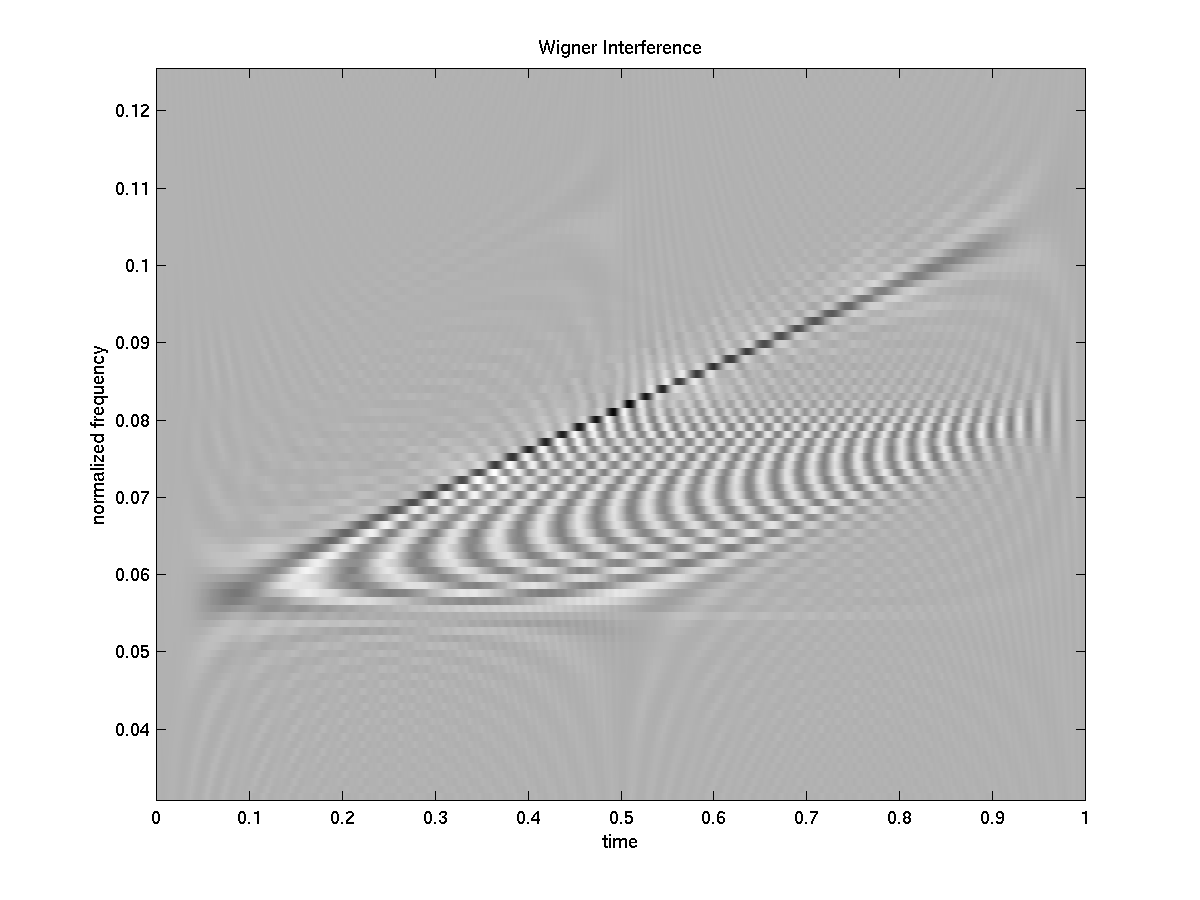
\includegraphics[width=7cm, height=6cm]{WVI}}
\caption{Wigner-Ville interference energy of a constant
  frequency modulation plus a linear chirp.}
\label{fig:WVI}
\end{center}
\end{figure}

\begin{figure}[htbp]
  \begin{center}
    \framebox[7cm]{\rule[-5mm]{0cm}{5cm}
  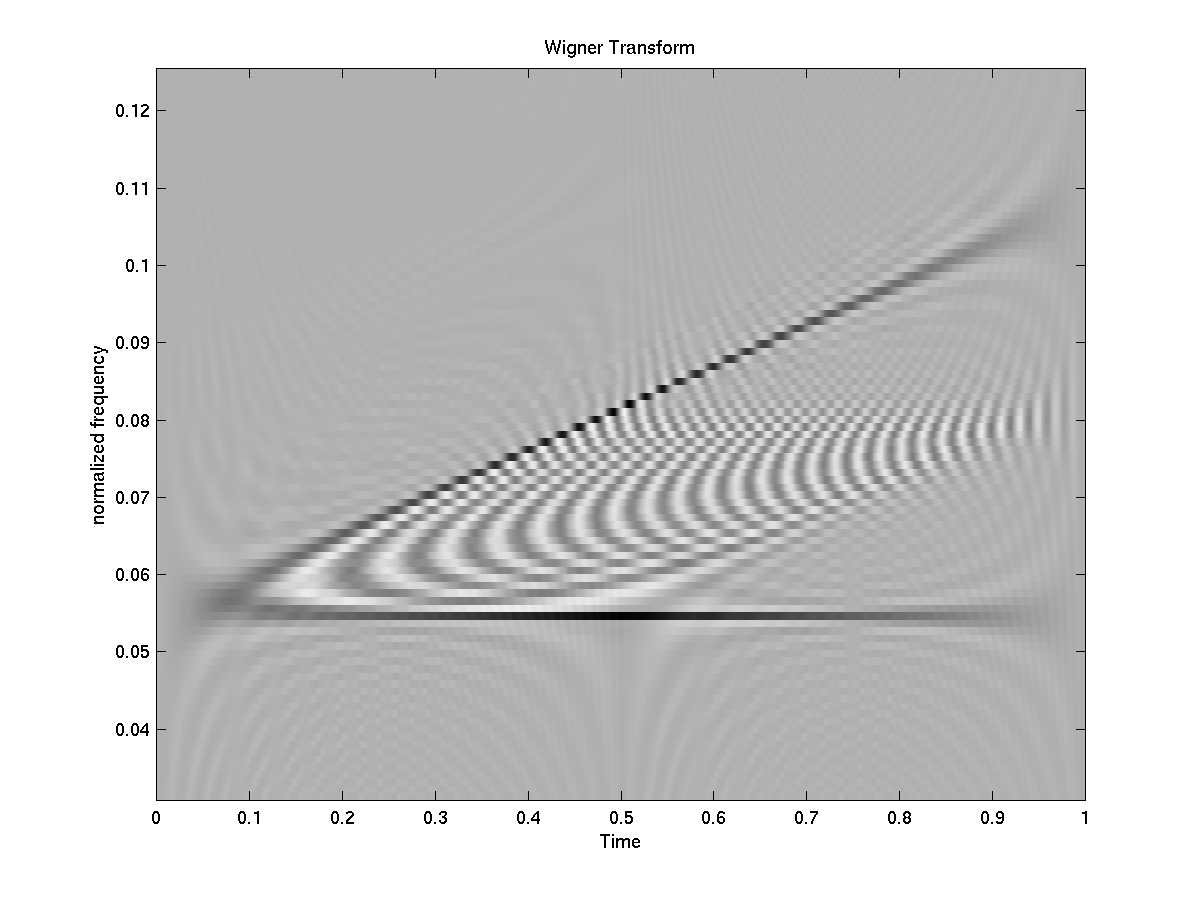
\includegraphics[width=7cm, height=6cm]{WVT}}
\caption{Wigner-Ville transform of a constant
  frequency modulation plus a linear chirp.}
\label{fig:WVT}
\end{center}
\end{figure}
}

The next section describes how we use the interference energy to derive a dissonance
measure of the signal.

\section{Dissonance Measures}
\def\tpull{\left(t+\halftau\right)}
\def\tpush{\left(t-\halftau\right)}
\def\I{\mathcal{I}}
\subsection{A Simple Dissonance Measure}
We first consider perhaps the simplest of the many possible dissonance measures
based on the information provided by the interference energy of the Wigner
transform. 

%Consider the function $\phi_{g_(\gamma_n}g_{\gamma_n}}(t,\tau)
Section~\ref{sec:wigner} introduced the function
$\phi_x(t,\tau)$.  Let's generalize this slightly by defining
\[
\phi_{g_{\gamma_m}g_{\gamma_n}}(t,\tau) 
= g_{\gamma_m}\tpull g^*_{\gamma_n}\tpush
\]
By definition of the cross \WT\ in equation~(\ref{eqn:crossWigner}),
$\W_{g_{\gamma_m}g_{\gamma_n}}$ is the Fourier transform of 
$\phi_{g_{\gamma_m}g_{\gamma_n}}(t,\tau)$ 
%$\phi_{m,n}$ 
with respect to $\tau$.  Therefore, the inverse Fourier 
transform of $\W_{g_{\gamma_m}g_{\gamma_n}}$ is
$\phi_{g_{\gamma_m}g_{\gamma_n}}$. 
%$\phi_{m,n}$.  
That is,
\[
\int
\W_{g_{\gamma_m}g_{\gamma_n}}(t,\nu) e^{i2\pi\nu\tau}\;d\nu
= \phi_{g_{\gamma_m}g_{\gamma_n}}(t,\tau) 
\]
Suppose that, at any given point in time, we integrate
$\W_{g_{\gamma_m}g_{\gamma_n}}(t,\nu)$ over all frequencies, $\nu$.  This is
equivalent to evaluating $\phi_{g_{\gamma_m}g_{\gamma_n}}$ at $\tau = 0$:
\begin{align}
\int
\W_{g_{\gamma_m}g_{\gamma_n}}(t,\nu)\;d\nu
&=\phi_{g_{\gamma_m}g_{\gamma_n}}(t,0)\nonumber \\
&= g_{\gamma_m}(t)g^*_{\gamma_n}(t) \label{eq:intWV}
\end{align}

As a first proposal, we consider measuring the dissonance at time $t$ of the
signal $x$ by integrating the interference energy
$I_x(t,\nu)$ over all frequencies $\nu$.  The result %in the continuous case,
is 
\begin{equation}\label{eq:specialI}
\I_x(t) = \int I_x(t,\nu)\; d\nu
\end{equation}
\[
=\sum_{m, n}
    \langle R^mx,g_{\gamma_m}\rangle \langle R^nx,g_{\gamma_n}\rangle^*
      \int \W_{g_{\gamma_m}g_{\gamma_n}}(t,\nu)\; d\nu
\]
%\[
%=2\sum_m\sum_{n>m}
%     \Real\left[\langle R^mx,g_{\gamma_m}\rangle \langle R^nx,g_{\gamma_n}\rangle^*
%        g_{\gamma_m}(t) g^*_{\gamma_n}(t)\right]
%\]
%Below we will see a graph of this measure for our %basic, yet revealing 
%example consisting of a sine tone plus a linear chirp. 

The lower graph in
Figure~\ref{fig:sIequal} shows how the function $\I_x(t)$ behaves for the
constant tone plus linear chirp.  The top graph is there for reference and
represents the value of the instantaneous frequencies of the signal.
Figure~\ref{fig:sIjust} also shows the value of $\I_x(t)$ for the example signal.
However, in this figure the time axes are delimited by tick marks representing
just and Pythagorean tunings. Table~\ref{table:ratios} presents the frequency
ratios corresponding to these tick marks.

%\begin{figure}[htbp]
%  \begin{center}
%    \framebox[7cm]{\rule[-5mm]{0cm}{5cm}
%  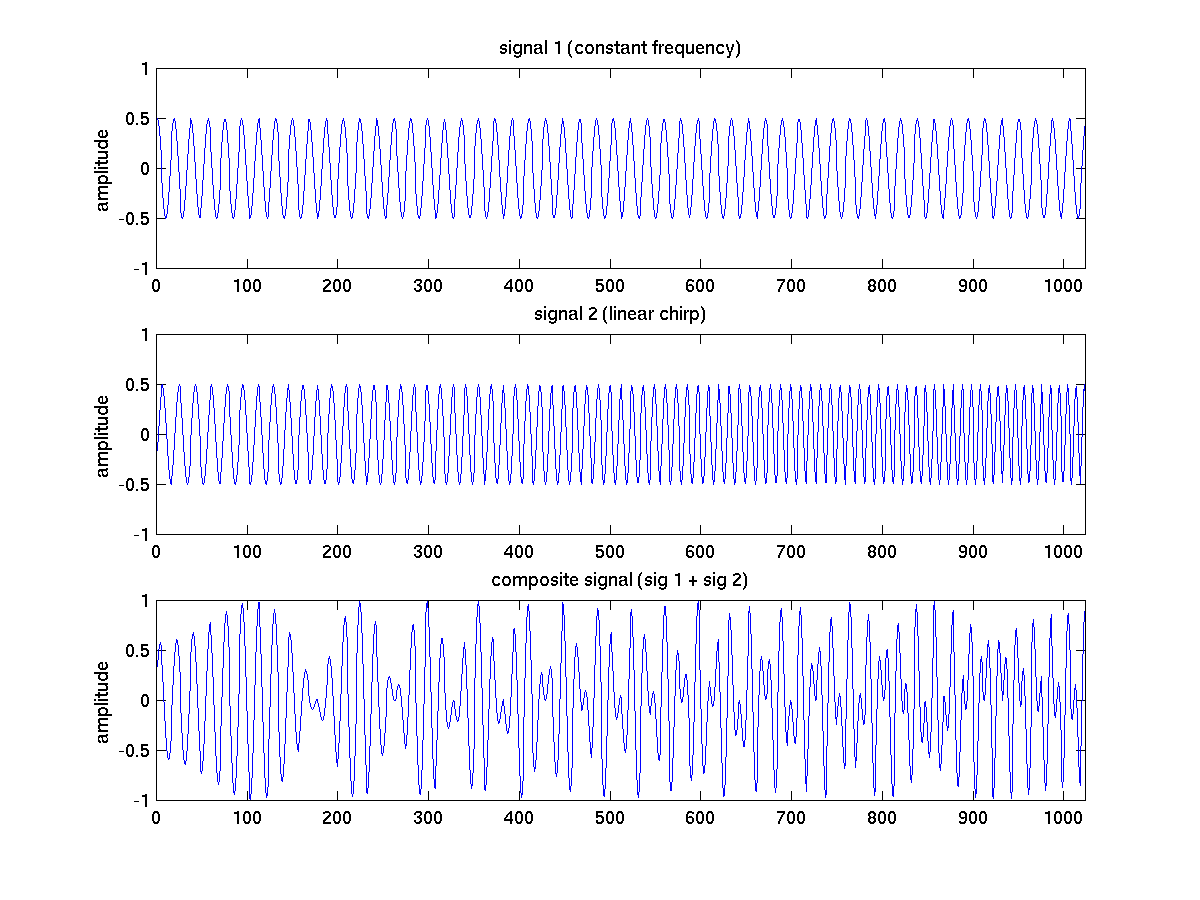
\includegraphics[width=7cm, height=6cm]{signal}}
%\caption{A constant frequency modulation plus a linear chirp.}
%\label{fig:signal}
%\end{center}
%\end{figure}

\ifthenelse{\boolean{nofigures}}{}{
\begin{figure}[htbp]
  \begin{center}
    \framebox[7cm]{\rule[-5mm]{0cm}{5cm}
  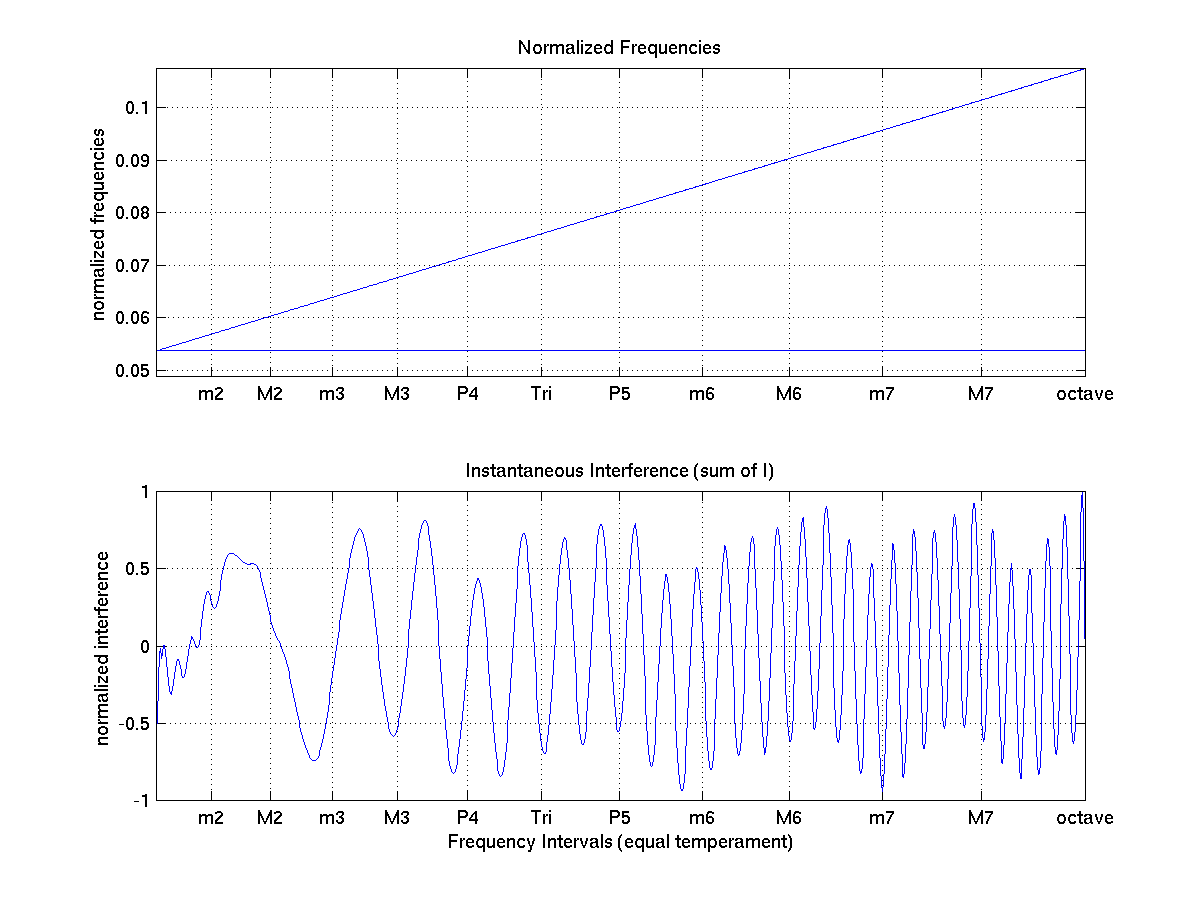
\includegraphics[width=7cm, height=6cm]{sumIequal}}
\caption{(a) Normalized instantaneous frequencies; (b) Instantaneous
  interference -- the sum of interferences at each point in time; the time
  axis of (b) is delimited by the ratio of the two frequencies in figure (a),
  with tick marks illustrating points of an equal tempered scale.}
\label{fig:sIequal}
\end{center}
\end{figure}
}
\begin{table}
  \begin{center}
%    \framebox[7cm]{\rule[-5mm]{0cm}{5cm}

\begin{tabular}{l|r|r|r}
Name & Just & Pythagorean & Equal\\
\hline
m2 &16/15& 256/243& $2^{1/12}$\\
M2 & 9/8 & 9/8& $2^{2/12}$\\
m3 &6/5 & 32/27& $2^{3/12}$\\
M3 &5/4 & 81/64& $2^{4/12}$\\
P4 &4/3 & 4/3& $2^{5/12}$\\
Tritone &64/45 & 729/512& $2^{6/12}$\\
P5 &3/2 & 3/2 & $2^{7/12}$\\
m6 &8/5&128/81& $2^{8/12}$\\
M6 & 5/3& 27/16 & $2^{9/12}$\\
m7 & 7/4& 16/9 & $2^{10/12}$\\
M7 & 15/8& 243/128 & $2^{11/12}$\\
octave& 2 & 2 & $2^{12/12}$
\end{tabular}
%}
\caption{Frequency ratios used to delimit the horizontal axis in the figures.}
\label{table:ratios}
\end{center}
\end{table}

\ifthenelse{\boolean{nofigures}}{}{
\begin{figure}[htbp]
  \begin{center}
    \framebox[7cm]{\rule[-5mm]{0cm}{5cm}
  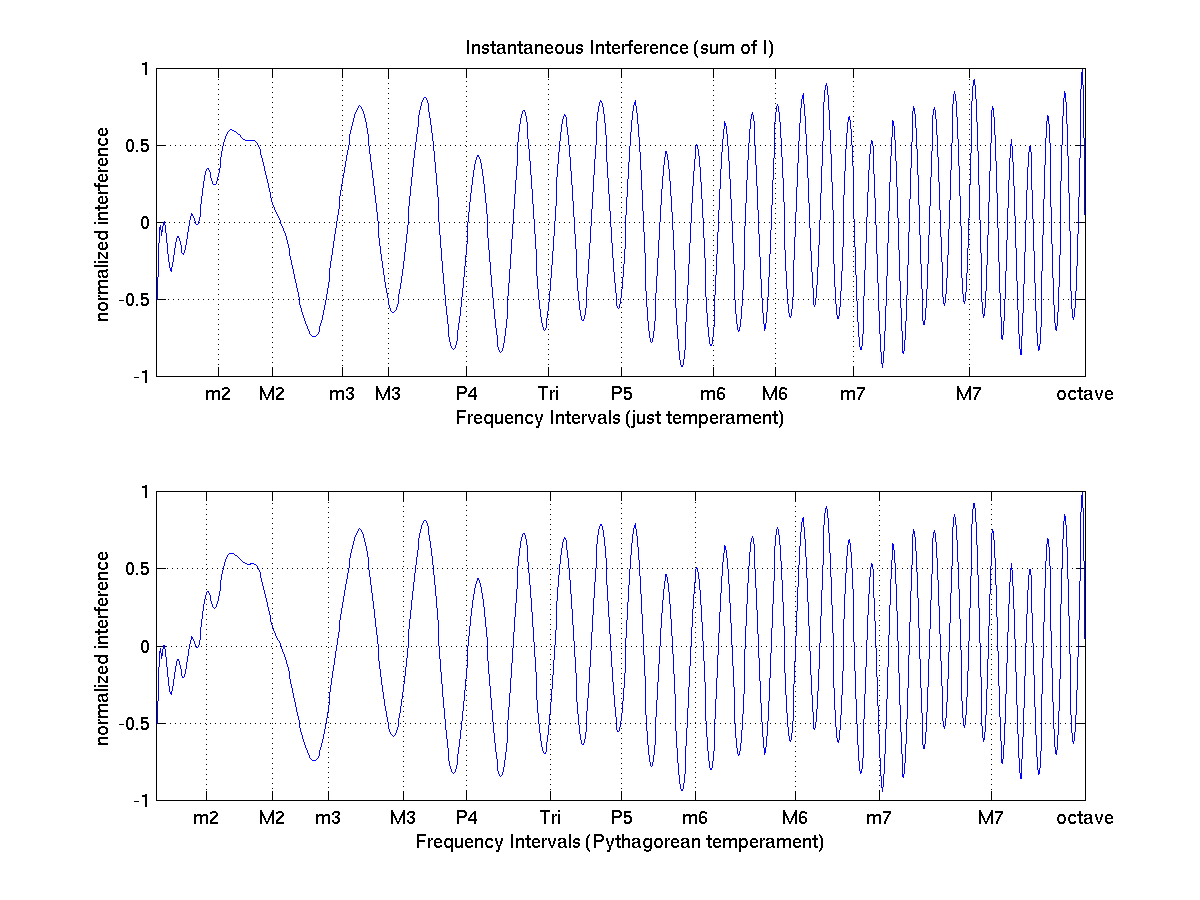
\includegraphics[width=7cm, height=6cm]{sumIjust}}
\caption{Instantaneous interference for just and Pythagorean tunings. This
  figure is the same as that of \ref{fig:sIequal} (b), except that the 
  tick marks illustrate points of a just (a) and Pythagorean (b) scale.}
\label{fig:sIjust}
\end{center}
\end{figure}
}

We first note that, in all three tuning systems, the perfect 5th falls in
roughly the same place, and that this interval consistently corresponds to
local minima of $\I_x(t)$. Other significant intervals, such as the major 3rd
and the tritone, also correspond to local minima of $\I_x(t)$.

\subsection{A General Dissonance Measure}
As stated at the outset, we want to find not only a point-wise measure of
dissonance, but also a measure that could account for melodic context.  The
function $\I_x(t)$ is essentially the sum over $\nu$ of the 
function $I_x(t,\nu)$.  Since $I_x(t,\nu)$ is a measure of interferences among
signal components centered at $t$ as well as those centered at times
surrounding $t$, it might seem as though the function $\I_x(t)$ accounts for
melodic context.  
However, note that
\[
\I_x(t) =\sum_{m,n}
      \langle R^mx,g_{\gamma_m}\rangle \langle R^nx,g_{\gamma_n}\rangle^*
        g_{\gamma_m}(t) g^*_{\gamma_n}(t)
\]
by equation~(\ref{eq:intWV}).
Thus $\I_x(t)$ only measures interferences among signal components at the
single time instant $t$. %, and it does not account for interferences occuring
%between atoms at different instances.  
Still, as the results for our simple example show, it may provide a useful
point-wise dissonance characterization of a signal.

We can generalize the foregoing by considering the inverse Fourier transform
of the interference energy:
%\begin{align*}
%\I_x(t,\tau) &= \int I_x(t,\nu)e^{i2\pi\nu\tau}\; d\nu\\
%&=\sum_{m, n} 
%\langle R^mx,g_{\gamma_m}\rangle \langle R^nx,g_{\gamma_n}\rangle^* \times\\
%&\quad \int \W_{g_{\gamma_m}g_{\gamma_n}}(t,\nu)e^{i2\pi\nu\tau}\; d\nu
%\end{align*}
%\end{align*}
%This is equivalent to
%\[
%\I_x(t,\tau) =\sum_{m, n} 
%\langle R^mx,g_{\gamma_m}\rangle \langle R^nx,g_{\gamma_n}\rangle^* 
%\phi_{g_{\gamma_m}g_{\gamma_n}}(t,\tau)
%\]
\[  
\I_x(t,\tau) = \int I_x(t,\nu)e^{i2\pi\nu\tau}\; d\nu  
\]
\[
= \sum_{m, n}\langle R^mx,g_{\gamma_m}\rangle \langle R^nx,g_{\gamma_n}\rangle^* 
\phi_{g_{\gamma_m}g_{\gamma_n}}(t,\tau)
\]
Recall,
\[
\phi_{g_{\gamma_m}g_{\gamma_n}}(t,\tau) 
= g_{\gamma_m}\tpull g^*_{\gamma_n}\tpush
\]
The function $\I_x(t,\tau)$ leads to dissonance measures based on interferences
between signal components at different points in time.  For instance, a measure
of interferences among signal components that are separated by not more than 
$\tau_0$ units of time is
\begin{align}\label{eq:indicatorDiss}
\I_x^{\tau_0}(t) &= \int_0^{\tau_0} \I_x(t,\tau)\; d\tau\\
&=\sum_{m, n} \langle R^mx,g_{\gamma_m}\rangle \langle
                      R^nx,g_{\gamma_n}\rangle^* \times \nonumber\\
&\quad \int_0^{\tau_0} g_{\gamma_m}\tpull g^*_{\gamma_n}\tpush\;d\tau\nonumber
\end{align}
Of course, we can vary $\tau_0$ depending on the extent to which we wish to
account for interferences among signal components across time. 

More generally, put a distribution $\mu$ on the domain of time differences
among signal components.  This distribution describes the
relative importance of the interferences across various time intervals.  Then define,
\begin{equation}\label{eq:generalDiss}
\I_x^{\mu}(t) = \integral \I_x(t,\tau)\; d\mu(\tau)
\end{equation}

The definition of $\I_x$ in equation~(\ref{eq:specialI}) and $\I_x^{\tau_0}$
in equation~(\ref{eq:indicatorDiss}) are special cases
of~(\ref{eq:generalDiss}). We arrive at $\I_x^{\tau_0}$ by setting
\[
d\mu(\tau) = \chi_{[0,\tau_0)}(\tau)\;d\tau
\]
where $\chi_{[0,\tau_0)}(\tau)$ is the characteristic function, equal to 1 when
$\tau \in [0,\tau_0)$ and 0 elsewhere. In this case, $\mu$ is a uniform
distribution of width $\tau_0$.  Therefore, $\mu$ assigns equal importance to
interferences among components separated by at most $\tau_0$ units of time,
and zero importance to interferences among components separated by more than
$\tau_0$ units. Clearly, by setting $\tau_0 = 0$ in the foregoing, we
  return to the simplest measure, $\I_x$, with which we began.

Figure~\ref{fig:Icorr} shows how the function $\I_x^{\tau_0}$ behaves for our
example signal and two values of $\tau_0$.  The upper graph shows
$\I_x^{\tau_0}$ for $\tau_0 = 5.9$ milliseconds, and the lower graph shows
the same function for $\tau_0 = 46.9$ milliseconds.  

One interesting aspect of these figures is the behavior they exhibit near
the perfect fifth interval.  Taken as a measure of dissonance, the figures
indicate that dissonance is high when the ratio approaches the perfect fifth
and low once it reaches the perfect fifth. 
%In fact, for $\tau_0 = 46.9$
%milliseconds, the perfect fifth acheives minimum dissonance.

\ifthenelse{\boolean{nofigures}}{}{
\begin{figure}[htbp]
  \begin{center}
    \framebox[7cm]{\rule[-5mm]{0cm}{5cm}
  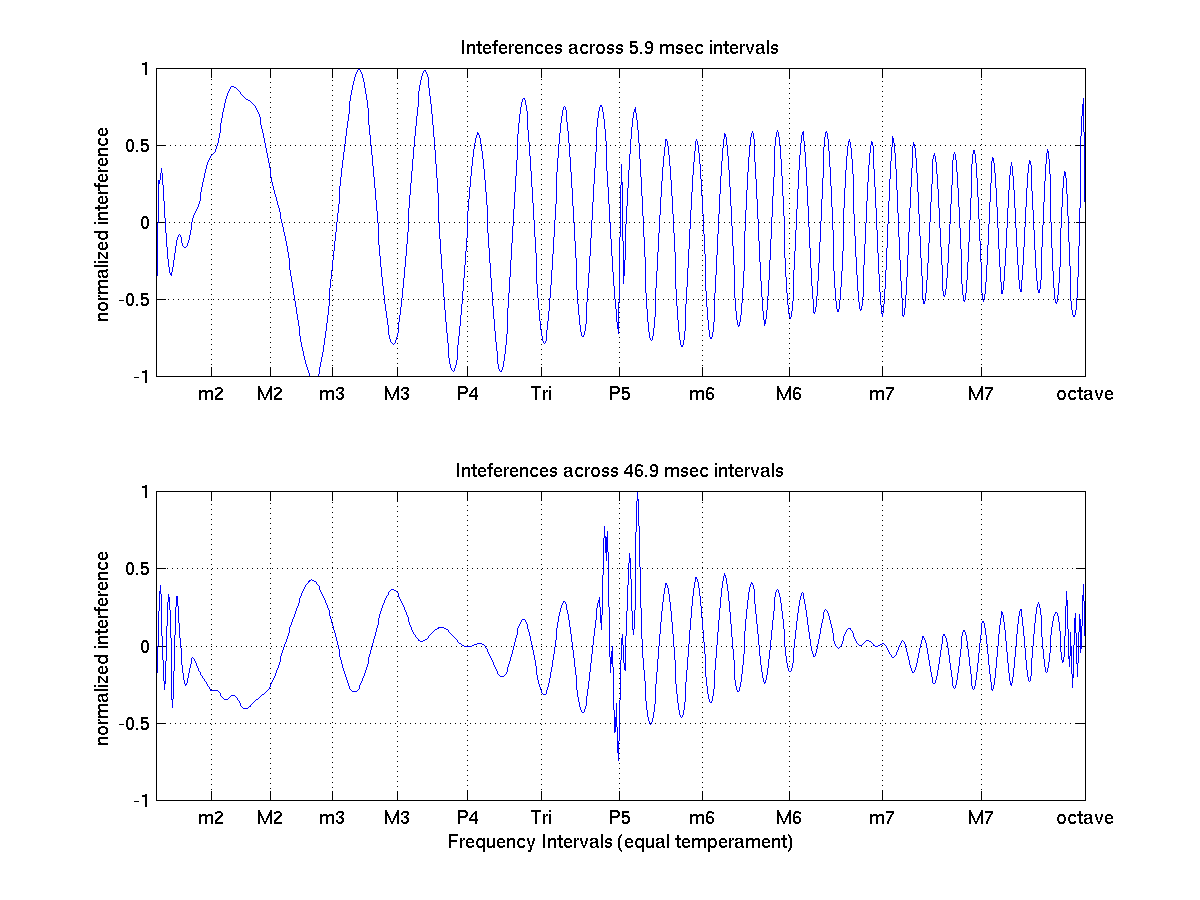
\includegraphics[width=7cm, height=6cm]{IcorrEqual}}
\caption{Interference measure $\I_x^{\tau_0}$; the sum of interferences over
  the given time intervals.}
\label{fig:Icorr}
\end{center}
\end{figure}
}

\section{Conclusion}
We have described the function, $I_x$, representing the sum of the
interference terms of the \WT\ of a signal. %, and we called this the
%interference energy of the signal.  
Based
on this function we derived a measure, $\I_x^{\tau_0}$, of interference among
signal components over a given interval of time, $\tau_0$.  Finally, we
proposed a general interference measure, $\I_x^{\mu}$, by putting a distribution
$\mu$ on the domain of time differences between signal components.  

The dissonance measure that results from the foregoing depends on the function
$\mu$, which represents the relative importance we place on interferences
across various time intervals.  Generalizing $\I_x$ is this way enables
the interference function to account for melodic context, and this provides
heuristic justification for the use of $\I_x^{\mu}$ as a measure of melodic
dissonance.

We have shown that the measures presented above exhibit interesting
behavior for our simple example.  However, it is as yet unclear exactly how
useful, as measures of dissonance,  %is the information provided by 
are such functions.  We expect that further research, and experience with
these functions in musical situations, will at least demonstrate their utility
as a means of characterizing musical signals.   

%%% Local Variables: 
%%% mode: latex
%%% TeX-master: "ICMC"
%%% End: 

% -*- mode: LaTeX; tex-main-file: "ICMC.tex"; -*-
\section{Analytic Interference}
\label{sec:analytic}
Reconsider the composite signal $x(t) = x_\a(t) + x_\b(t)$, where
\[
x_\a(t)
      =e^{i2\pi(\nu_m-\halfDnu)t},\;
x_\b(t)
      = e^{i2\pi(\nu_m+\halfDnu)t}
\]
%The \WT\ of $x(t)$ is 
%\[  \W_{x_\a+x_\b}(t,\nu) = \W_{x_\a}(t,\nu)+\W_{x_\b}(t,\nu) + I_{x_\a x_\b}(t,\nu)\]\[ =\delta(\nu-(\nu_m-\halfDnu))+\delta(\nu-(\nu_m+\halfDnu))\]\[+ \delta(\nu-\nu_m)\,2\cos(2\pi \Delta\nu t)\]
%Therefore, t
The interference energy is %given by
\[
I_x(t,\nu) = \delta(\nu-\nu_m)\,2\cos(2\pi \Delta\nu t)
\]
Integrating,
\begin{align*}
%\I_x(t) &= \int \delta(\nu-\nu_m)\,2\cos(2\pi \Delta\nu t) \,d\nu\\
\I_x(t)   &= 2\cos(2\pi \Delta\nu t) \int \delta(\nu-\nu_m)\,d\nu\\
           &= 2\cos(2\pi \Delta\nu t)
\end{align*}

To simplify notation, let an atom in the dictionary be  denoted $g_n$.
Recall that, for an arbitrary linear combination of atoms, 
\[
x(t) = \sum_{n=0}^\infty \alpha_n g_n
\]
the interference energy is given by 
\[
I_x(t,\nu) = \sum_{n=0}^\infty \sum_{m=0}^\infty \alpha_n\alpha_m^*W_{g_ng_m}(t,\nu)
\]
and, under suitable conditions which permit interchanging the summation and integration,
\begin{align*}
\I_x(t) &= \sum_{n=0}^\infty \sum_{m=0}^\infty \alpha_n\alpha_m^*\int W_{g_ng_m}(t,\nu) \, d\nu\\
&= \sum_{n=0}^\infty \sum_{m=0}^\infty \alpha_ng_n(t)\overline{\alpha_m g_m}(t)
\end{align*}


%\bibliographystyle{IEEEbib} %\bibliographystyle{ieeetr}
\bibliographystyle{chicago}
\small{
\bibliography{icmc2002}
}

\end{document}
